\documentclass{article}
\usepackage{arxiv}
%\usepackage[fontset=windows]{ctex} 
\usepackage[utf8]{inputenc} % allow utf-8 input
\usepackage[T1]{fontenc}    % use 8-bit T1 fonts
\usepackage{hyperref}       % hyperlinks
\usepackage{url}            % simple URL typesetting
\usepackage{booktabs}       % professional-quality tables
\usepackage{amsfonts}       % blackboard math symbols
\usepackage{nicefrac}       % compact symbols for 1/2, etc.
\usepackage{microtype}      % microtypography
\usepackage{lipsum}		% Can be removed after putting your text content
\usepackage{graphicx}
%\usepackage{natbib}
\usepackage{doi}
\usepackage{amsmath}
\usepackage{graphicx}
\usepackage{subfigure}
\usepackage{float} % 加载 float 宏包
\usepackage{color}

\usepackage{hyperref}
\usepackage[style=authoryear,backend=biber]{biblatex}
\addbibresource{references.bib}  % 你的参考文献文件
% 让作者姓名在引用时成为超链接
\DeclareCiteCommand{\textcite}
  {\boolfalse{citetracker}%
   \boolfalse{pagetracker}%
   \usebibmacro{prenote}}
  {\usebibmacro{citeindex}%
   \printtext[bibhyperref]{\printnames{labelname}}%
   \setunit{\addcomma\space}%
   \printtext[bibhyperref]{\printfield{year}}}
  {\multicitedelim}
  {\usebibmacro{postnote}}
  
\title{Application of Finite Element Methods in Solving PDE-Constrained Optimization for Heat Conduction Problems}

%\date{September 9, 1985}	% Here you can change the date presented in the paper title
%\date{} 					% Or removing it

\author{ \href{}{
\includegraphics[scale=0.06]{orcid.pdf}\hspace{1mm}Yifan Cai}\\
	Computer Science\\
        2021533087\\
	ShanghaiTech\\
	\texttt{caiyf@shanghaitech.edu.cn} \\
	%% examples of more authors
	\And
	\href{}{
\includegraphics[scale=0.06]{orcid.pdf}\hspace{1mm}Peijun Xu} \\
Computer Science\\
        2021533041\\
	ShanghaiTech\\
	\texttt{xupj1@shanghaitech.edu.cn} \\
 \And
	\href{}{
\includegraphics[scale=0.06]{orcid.pdf}\hspace{1mm}Fanhao Bu} \\
Computer Science\\
        2021533039\\
	ShanghaiTech\\
	\texttt{bufh@shanghaitech.edu.cn} \\
	%% \AND
	%% Coauthor \\
	%% Affiliation \\
	%% Address \\
	%% \texttt{email} \\
	%% \And
	%% Coauthor \\
	%% Affiliation \\
	%% Address \\
	%% \texttt{email} \\
	%% \And
	%% Coauthor \\
	%% Affiliation \\
	%% Address \\
	%% \texttt{email} \\
}

% Uncomment to remove the date
%\date{}

% Uncomment to override  the `A preprint' in the header

\renewcommand{\headeright}{Final Report}
\renewcommand{\undertitle}{Everyone has the same level of contribution}
\renewcommand{\shorttitle}{Computer Science And Engineering}

%%% Add PDF metadata to help others organize their library
%%% Once the PDF is generated, you can check the metadata with
%%% $ pdfinfo template.pdf

\begin{document}
    \maketitle
    \vspace{6em} % 设置摘要与标题的间距
    \normalsize % 设置正文字号
    % 摘要部分
    
    \begin{abstract}

    PDE-constrained optimization involves partial differential equations (PDEs) and optimization, playing crucial role in modeling and solving complex real-world problems. It is widely applied across various fields, especially in optimization design, optimal control, and inverse problems like parameter estimation. This paper focuses on the Simultaneous Analysis and Design (SAND) method and its application in specific types of PDE-constrained optimization problems (with FEM-like methods). Through three thermodynamics cases involving heat conduction in conductors, we address issues such as temperature distribution fitting and internal heat source prediction.
    Our paper is mainly inspired by the Finite Element chapter in the Computational Science and Engineering course and the Convex Optimization section in the Numerical Optimization course, and extends the content of FEM to further read the relevant literature on Finite Element Tearing and Interconnect (FETI). 

    It is worth mentioning that all the code designs related to this paper are original to our team, with no borrowing or referencing from existing works. The overall approach of this paper is to practically apply algorithms to specific thermodynamic case studies after thoroughly understanding the relevant field. Although it does not present entirely new and innovative ideas, it includes our own insights and expansion attempts. This paper aims to emphasize the important role of effective numerical techniques in real-life applications. Through this discussion, we hope to gain deeper insights into Computational Science and Engineering, particularly in the field of Finite Element optimization problem-solving, and ultimately apply these insights effectively in our practical work and research.
    \end{abstract}
    \keywords{PDE \and Thermal Conduction Problem \and Control Optimization Theory}
    \clearpage % 换页
    
    % 正文部分
    % Part one
    \section{Problem Background And Restatement}
    \subsection{SAND Methods (Simultaneous Analysis and Design)}
    The application of the Simultaneous Analysis and Design (SAND) method in PDE-constrained optimization problems has attracted significant attention and in-depth research in recent years. Compared with the traditional Nested Analysis and Design (NAND) method, the core idea of the SAND method is to integrate the solution of partial differential equations (PDEs) with the optimization process, addressing both issues simultaneously rather than handling them separately. 
    
    In recent years, researchers have developed many advanced algorithms and techniques for the SAND method. Multigrid Methods (\textcite{MultigridMethods} ) accelerate the solution process by utilizing information on different grid scales, and Preconditioning Techniques (\textcite{Preconditioningiterativemethods}) transform the original problem into an equivalent but easier-to-solve system by improving the condition number of the matrix, thus enhancing the convergence speed of iterative methods. These have been widely applied to improve computational efficiency and demonstrate excellent performance in handling large-scale and complex PDE-constrained optimization problems.

    In combination with this article, we integrating the basic knowledge of convex optimization with finite element methods, striving to achieve a comprehensive understanding of the knowledge learned. We embeds the PDE solution process into the optimization, thereby reducing computational overhead and time consumption, significantly enhancing computational efficiency. This paper will focus on using the SAND method and concentrate on one particular type of PDE-constrained optimization problem: optimal control.

    
    
    \subsection{One-Dimensional Steady-State Heat Conduction Differential Equation}
    This paper mainly explores the application of FEM and Convex Optimization algorithms in the field of thermodynamics, so we need to firstly clarify the basic principle of heat conduction.
    
    According to Fourier's Law(\textcite{Phisics}): The direction of heat flow is always from the high-temperature region to the low-temperature region, and the magnitude of the heat flow is proportional to the temperature gradient. The direction of the heat flow is opposite to the direction of the temperature gradient. we let \( f(x) \) represents the heat flux or the internal heat source term, where x$\in$ X (X is the length of conductor) , $u(x)$ represent the temperature distribution on the conductive conductor, and  \( k(x) \) is the thermal conductivity, which may be a function of position or can simplify to an constant. The Fourier's Law formula can be expressed as:
      \begin{equation}
          f(x) = -k(x) \frac{du}{dx}
      \end{equation}

    In steady-state conditions, the net heat flow through a differential cross-section $dx$ is equal to the heat generated internally. To express this mathematically for a small segment $dx$, we can substitute Fourier's law into the energy conservation equation. This substitution yields a comprehensive expression of energy conservation as follows:
    \begin{equation}
         \frac{d}{dx} \left( k(x) \frac{du}{dx} \right) + f(x) = 0
    \end{equation}

Where $\frac{d}{dx} \left( k(x) \frac{du}{dx} \right) $ represents the spatial variation of the heat flux. For constant thermal conductivity \( k \) (which is our paper mainly focused on), this simplifies to the one-dimensional steady-state heat conduction differential equation:

\begin{equation}
    k \frac{d^2 u}{dx^2} + f(x) = 0
\end{equation}

The one-dimensional steady-state heat conduction differential equation in \textcite{heat} 
 describes the rate of heat generation at various points inside a conductor, which may be a function of position variation. The second derivative of the temperature distribution \( u \) is proportional to the internal heat source distribution \( f \).  Easy to find, the internal heat source will affect the temperature distribution inside the conductor, but it will not change the set boundary temperature, so we can further define the temprature at two ends later. 


In this paper, the thermal conductivity \( k \) is always a constant, and for the sake of convenience, we further define it as 1, i.e. 
\begin{equation}
    - u''(x) = f(x)
\end{equation}
Solving this equation requires appropriate boundary conditions. Common boundary conditions include:

\begin{enumerate}
    \item \textbf{Dirichlet Boundary Condition (Constant Temperature):} The temperature at the boundary is known, for example, \( T(0) = T_0 \) and \( T(L) = T_L \).
    \item \textbf{Neumann Boundary Condition (Constant Heat Flux):} The heat flux at the boundary is known, for example,
    \[
    \frac{dT}{dx} \bigg|_{x=0} = q_0
    \]
    \item \textbf{Convective Boundary Condition:} Heat transfer at the boundary through convection with the surrounding environment, for example,
    \[
    -k \frac{dT}{dx} \bigg|_{x=L} = h(T(L) - T_\infty)
    \]
\end{enumerate}

Depending on the specific problem, these differential equations can be solved using integration or numerical methods.

\subsection{KKT Conditions And Lagrange Multipliers In Convex Optimization Problems}

In convex optimization problems, the Karush-Kuhn-Tucker (KKT) conditions and the Lagrange multipliers method are two essential tools for handling constrained optimization problems (\textcite{convex}). 

The Lagrange multipliers method is used to solve optimization problems with equality constraints. Considering the objective function \(f(x)\) and the equality constraints \(h_i(x) = 0, \ i = 1, \ldots, m\), the Lagrangian function can be constructed as follows:

\[
L(x, \lambda) = f(x) + \sum_{i=1}^{m} \lambda_i h_i(x),
\]

where \(\lambda_i\) are the Lagrange multipliers. The key to solving this optimization problem is to find the points where the first-order partial derivatives of the Lagrangian function are zero, which are the candidate solutions.
    \[
    \nabla_x L(x, \lambda) = 0 \quad \text{and} \quad h_i(x) = 0, \ i = 1, \ldots, m.
    \]

The KKT conditions are an extension of the Lagrange multipliers method. Considering the objective function \(f(x)\), the equality constraints \(h_i(x) = 0\), and the inequality constraints \(g_j(x) \leq 0\), the problem can be formulated as follows:
\begin{equation}
    \begin{cases}
        min \, f(x)\\
        s.t. \,  h_i(x) = 0, \ i = 1, \ldots, m\\
        \,\, \ g_j(x) \leq 0, \ j = 1, \ldots, p.
    \end{cases}
\end{equation}
The Lagrangian Function is:
    \[
    L(x, \lambda, \mu) = f(x) + \sum_{i=1}^{m} \lambda_i h_i(x) + \sum_{j=1}^{p} \mu_j g_j(x),
    \]
    where \(\lambda_i\) and \(\mu_j\) are the Lagrange multipliers for the equality and inequality constraints, respectively.
Then the Stationarity Condition becomes:
    \[
    \nabla_x L(x, \lambda, \mu) = \nabla f(x) + \sum_{i=1}^{m} \lambda_i \nabla h_i(x) + \sum_{j=1}^{p} \mu_j \nabla g_j(x) = 0.
    \]
\begin{enumerate}
    \item \textbf{Complementary Slackness Condition}:
    \[
    \mu_j g_j(x) = 0, \ j = 1, \ldots, p.
    \]
    \item \textbf{Non-Negativity Condition}:
    \[
    \mu_j \geq 0, \ j = 1, \ldots, p.
    \]
    \item \textbf{Feasibility Condition}:
    \[
    h_i(x) = 0, \ i = 1, \ldots, m,\ \text{and} \ g_j(x) \leq 0, \ j = 1, \ldots, p.
    \]
\end{enumerate}

The KKT conditions provide a set of necessary and sufficient conditions for determining whether a solution is optimal in convex optimization problems. Due to the property of convexity, these conditions are not only necessary but also sufficient, which simplifies and enhances the efficiency of the solution process.


\subsection{Introduction To the Finite Element Method (FEM)}

The Finite Element Method (FEM) is a numerical technique for finding approximate solutions to boundary value problems for partial differential equations. It is widely used in engineering, physics, and applied mathematics for simulating physical systems. The core idea of FEM is to decompose a complex problem domain into simpler parts, called finite elements, and then formulate the problem as a system of algebraic equations (\textcite{FEM}).

FEM involves dividing the domain of the problem into a finite number of subdomains, called segments, which are connected at discrete points known as nodes. The solution to the problem is approximated within each element using simple polynomial functions. The overall solution is obtained by assembling the solutions of all elements and ensuring continuity at the nodes.

\begin{enumerate}
    \item \textbf{Discretization}: The domain is divided into smaller, non-overlapping elements. Common element shapes include triangles, quadrilaterals, tetrahedra, and hexahedra.
    \item \textbf{Selection of Shape Functions}: Within each element, the solution is approximated using shape functions, which are typically polynomials. These functions are chosen to satisfy certain properties, such as continuity across element boundaries.
    \item \textbf{Formulation of Element Equations}: The differential equation governing the problem is transformed into an equivalent variational form, usually involving integrals. This is done by multiplying the differential equation by a test function and integrating over the domain. The result is a set of algebraic equations for each element.
    \item \textbf{Assembly of Global System}: The local element equations are assembled into a global system of equations that represents the entire problem. This system incorporates boundary conditions and interactions between elements at the nodes.
    \item \textbf{Solution of the Global System}: The global system of equations is solved using numerical methods to obtain the approximate solution to the original problem. 
\end{enumerate}
In this paper, we mainly use FEM to simulate heat distribution and temperature fields within objects(\textcite{PDE_t}).

    
    % Part Two
    \section{Problem Analysis}
    \subsection{A Basic Toy Problem}
    \subsubsection{Mathematical Derivation}
   Firstly, we consider a basic problem of heat conduction in a one-dimensional space: Suppose we have a heat-conducting iron rod of unit length i.e. 1. The temperatures at both ends of the rod are constant and denoted by Q, and there is an internal heat source term f(x). Assume there exists a real unknown temperature distribution u(x) along the rod, our goal is to calculate a function $u_{h}(t)$ to approach the real distribution. According to the One-Dimensional Steady-State Heat Conduction Differential Equation which has been mentioned in Chapter 1, we can obtain the equation about u(x):
    \begin{equation}
        -u''(x)=f(x)\label{basic formula}
    \end{equation}
    Our ultimate goal is to get a suitable approximation function $u_h(x)$ using a series of basis functions $\phi_i(x)$. First of all, we divide the rod into $n$ equal segments, with endpoints denoted as $\{$ $X_0$, $X_1$, $\ldots$, $X_n$$\}$.  Base on this division, in order to express any value in the spanned space through this series of basis functions, We designed a set of basis functions $\{$$\phi_0$, $\phi_1$, ..., $\phi_n $ $\}$ such that they can represent any value in the spanned space. Unlike the conventional definition of basis functions, in order to expand the scope and depth of our problem, we do not assume the presence of zero constraints at both ends of the rod, thus, we need to add two 'half' basis functions: $\phi_0(x)$, $\phi_n(x)$. The basis functions definitions are as follow:

    \begin{equation}
    \phi_{0}(x) =
    \begin{cases}
        \frac{X_{1}-x}{X_{1}-X_{0}}\: ,\: X_{0}\leq x\le X_{1}\\
        0 \: ,\: x < X_{0} \cup x>X_{1}
    \end{cases}
    \end{equation}
    
    \begin{equation}
        \phi_{i}(x) =
    \begin{cases}
        \frac{x-X_{i-1}}{X_{i}-X_{i-1}} \: ,\: X_{i-1}\leq x<X_{i}\\
        \frac{X_{i+1}-x}{X_{i+1}-X_{i}} \: ,\: X_{i}\leq x\le X_{i+1}\\
        0 \: ,\: x < X_{i-1} \cup x>X_{i+1}
    \end{cases}
    (1\le i\le n-1)
    \end{equation}
        \begin{equation}
        \phi_{n}(x) =
        \begin{cases}
            \frac{x-X_{n-1}}{X_{n}-X_{n-1}}\: ,\: X_{n-1}\leq x\le X_{n}\\
        0 \: ,\: x < X_{n-1} \cup x>X_{n}
        \label{basis function}
        \end{cases}
    \end{equation}
    
    \begin{figure}[H]
        \centering % 图片居中
        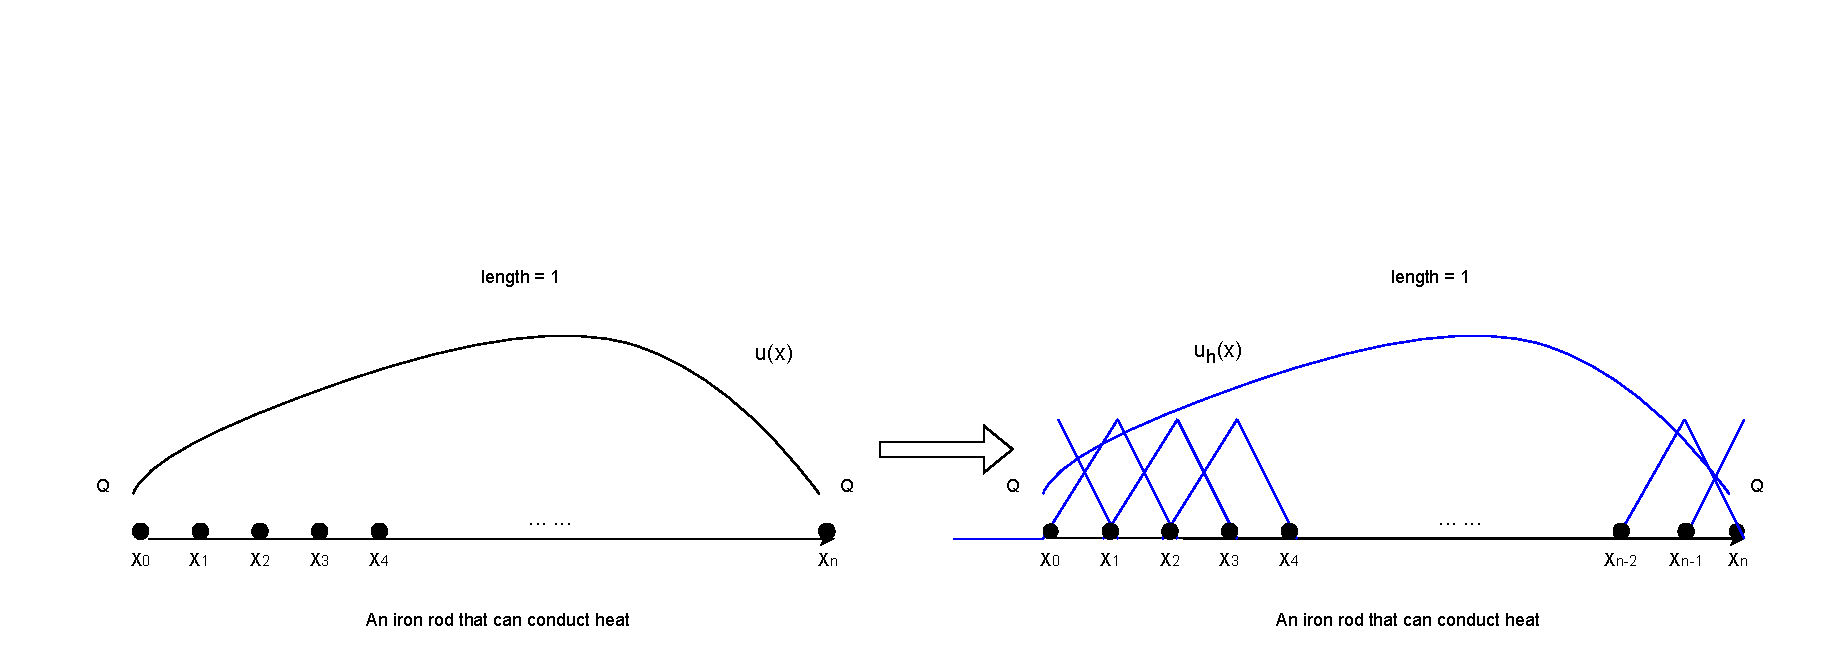
\includegraphics[width=16cm]{pic/1.drawio.pdf} % width设置图片大小
        \caption{As shown in the figure, we first divide the rod evenly into $n$ parts, and then use the linear combination of basis functions $\phi(x)$ to get fitting function $u_h(x)$ and to approximate the actual temperature distribution $u(x)$.
} % 设置图片的标题及引用标签
        \label{pic_1}
    \end{figure}
    
   The fitting function $u_h(x)$ should entirely lie within the space spanned by the basis functions and can be simply represented as a linear combination of the basis functions:
   \begin{equation}
       u_h(x)=u_{0}\phi_{0}(x)+u_{1}\phi_{1}(x)+...+u_{n}\phi_{n}(x) \label{u(x)}
   \end{equation}
    Where $\{$ $u_0$ ,$u_1$ , ..., $u_n$ $\}$ are the unknown weights of the basis functions. Now, our task is to approximate \( u(x) \) using \( u_h(x) \). Due to the limited smoothness of $u_{h}(x)$, we can obtain the weak form of the problem by multiplying both sides with a test function 
     \( v(x) = v_{0}\phi_{0}(x)+v_{1}\phi_{1}(x)+...+v_{n}\phi_{n}(x) \) and integrating over the entire domain. This allows us to handle cases where the function and its derivatives are discontinuous. The basic formula \ref{basic formula} now is changed into:

    \begin{equation}
        \int_{0}^{1} -u_{h}''(x)* v(x)  \, dx \,=\,\int_{0}^{1} f(x)*v(x)\,dx
    \end{equation}
    By 'Partial integration method', we can simplify and obtain:
    \begin{equation}
         \int_{0}^{1} u_{h}'(x)* v'(x)  \, dx \,-\,(u_{h}'(x)*v(x))\rvert_{\text{0}}^{\text{1}}=\,\int_{0}^{1} f(x)*v(x)\,dx \label{partial interate}
    \end{equation}
    Substitute formula \ref{u(x)} into the expression \ref{partial interate}, the formula becomes:
    \begin{equation}
         \int_{0}^{1} u_0\phi_0'(x)* v'(x)+...+u_{n}\phi_n'(x)* v'(x)  \, dx -\,( u_0\phi_0'(x)* v(x)+...+u_{n}\phi_n'(x)* v(x))\rvert_{\text{0}}^{\text{1}}=\int_{0}^{1} f(x)*v(x)\,dx \label{final equation}
    \end{equation}
    Since \( v(x) \) is also in the function space spanned by \{\( \phi_0 \) , \( \phi_1 \)... ... \( \phi_n \)\}, we further substitute the expression of v into formula \ref{final equation}, due to the linear independence of basis functions, the values in each basis direction should be equal, formula \ref{final equation} can be divided and rewritten into \( n \) equations:
     \begin{multline}
    \begin{cases}
        \int f(x)\phi_0(x) = u_0*\int \phi_0'(x)*\phi_0'(x)+ u_1*\int \phi_1'(x)*\phi_0'(x)+... ... +u_n*\int \phi_n'(x)*\phi_0'(x)\\-(u_0*\phi_0'(x)*\phi_0(x)+u_1*\phi_1'(x)*\phi_0(x)+...+u_n\phi_n'(x)*\phi_0(x)\rvert_{\text{0}}^{\text{1}}\\
        \\
        \int f(x)\phi_1(x) = u_0*\int \phi_0'(x)*\phi_1'(x) +u_1*\int \phi_1'(x)*\phi_1'(x) + ... ... +u_n*\int \phi_n'(x)*\phi_1'(x)\\-(u_0*\phi_0'(x)*\phi_1(x)+u_1*\phi_1'(x)*\phi_1(x)+...+u_n\phi_n'(x)*\phi_1(x)\rvert_{\text{0}}^{\text{1}}\\
        ... ... \\
        \int f(x)\phi_n(x) = u_0*\int \phi_0'(x)*\phi_n'(x) +  u_1*\int \phi_1'(x)*\phi_n'(x) +... ... +u_n*\int \phi_n'(x)*\phi_n'(x)\\-(u_0*\phi_0'(x)*\phi_n(x)+u_1*\phi_1'(x)*\phi_n(x)+...+u_n\phi_n'(x)*\phi_n(x)\rvert_{\text{0}}^{\text{1}}
    \end{cases}
    \end{multline}
    Let \( a(u, v) := (u', v') \), where \((-, -)\) denotes the \( L^2 \) inner product, we obtain the final matrix equation. From left to right, they are similar to the stiffness matrix K, solution u, and vector f that taught in class :
    \begin{multline}
        \begin{pmatrix}
            a(\phi_0,\phi_0)-(\phi_0'(x)*\phi_0(x))\rvert_{\text{0}}^{\text{1}} & a(\phi_1,\phi_0)-(\phi_1'(x)*\phi_0(x))\rvert_{\text{0}}^{\text{1}} & ...& a(\phi_n,\phi_0)-(\phi_n'(x)*\phi_0(x))\rvert_{\text{0}}^{\text{1}} \\
            a(\phi_0,\phi_1)-(\phi_0'(x)*\phi_1(x))\rvert_{\text{0}}^{\text{1}} & a(\phi_1,\phi_1)-(\phi_1'(x)*\phi_1(x))\rvert_{\text{0}}^{\text{1}} & ... & a(\phi_n,\phi_1)-(\phi_n'(x)*\phi_1(x))\rvert_{\text{0}}^{\text{1}} \\
            ... \\
            a(\phi_0,\phi_n) -(\phi_0'(x)*\phi_n(x))\rvert_{\text{0}}^{\text{1}}& a(\phi_1,\phi_n) -(\phi_1'(x)*\phi_n(x))\rvert_{\text{0}}^{\text{1}}& ...& a(\phi_n,\phi_n)-(\phi_n'(x)*\phi_n(x))\rvert_{\text{0}}^{\text{1}} \\
        \end{pmatrix} * \\
        \begin{pmatrix}
            u_0\\
            u_1\\
            ...\\
            u_n
        \end{pmatrix}
        = 
        \begin{pmatrix}
            (f(x) , \phi_0(x))\\
            (f(x) , \phi_1(x))\\
            ... ...\\
            (f(x) , \phi_n(x))\\
        \end{pmatrix} \label{matrix form}
    \end{multline}
    Since $\phi$, $f$ are given functions, $u$ can be easily calculated by Matlab. After we get vector $u$, we simply calculate :
    \begin{equation}
        u_h(x)=
        \begin{pmatrix}
            u_0\\
            u_1\\
            ...\\
            u_n
        \end{pmatrix}^T
        \begin{pmatrix}
            \phi_0(x)\\
            \phi_1(x)\\
            ...\\
            \phi_n(x)
        \end{pmatrix}
    \end{equation}
    The basic toy problem is perfectly solved.
    \subsubsection{Matlab Coding}
    After conducting theoretical analysis, we will proceed with coding specific cases and verify the accuracy of the output through practical calculations. We assume u(0) = u(1) to be 5, the internal heat source distribution $f(x)=-x^2+x+1$ (see figure \ref{pic_2}). Thus, a feasible real temperature distribution should be $u(x) = \frac{1}{12}x^4-\frac{1}{6}x^3-\frac{1}{2}x^2+\frac{7}{12}+5$. Further on, the pole is divide evenly into 100 segments and the basis function are strictly follow the definition defined in formula \ref{basis function} .
    \begin{figure}[H]
        \centering % 图片居中
        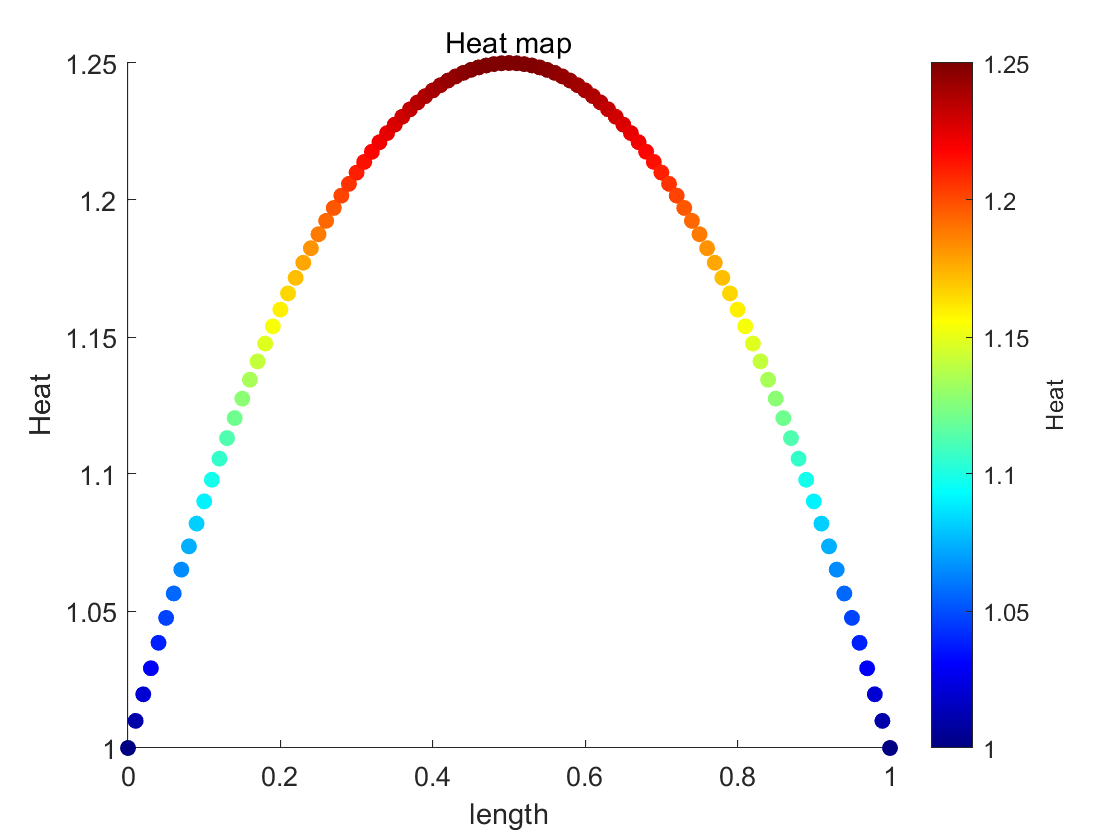
\includegraphics[width=11cm]{pic/heat.png} % width设置图片大小
        \caption{The internal heat source distribution $f(x)=-x^2+x+1$} % 设置图片的标题及引用标签
        \label{pic_2}
    \end{figure}
    
    A hard task we met is the need of values of $\phi_0'(0)$, $\phi_{n}'(1)$, $\phi_1'(0)$ and $\phi_{n-1}'(1)$ (see Fig.\ref{pic_3}), since we define to special basis function at both ends to ensure non-zero boundary constraint conditions. We find the shape of the function at each of these points is very specific and these are points where the function is not differentiable, so we need some special methods to handle their derivative values. 
    For the derivatives at points $\phi_0(0)$ and $\phi_{n}(1)$, since there are no functions defined on the left side of point $\phi_0(0)$ and the right side of point $\phi_{n}(1)$, we can only use the $\phi_0'(0+)$ for $\phi_0(0)$ and $\phi_{n}'(1-)$ for $\phi_{n}(1)$ as the derivatives at points $\phi_0(0)$ and $\phi_{n}(1)$, respectively. As for the derivatives at points $\phi_1(0)$ and $\phi_{n-1}(1)$, we define $\phi_1'(0)=\frac{\phi_1'(0+)+\phi_1'(0-)}{2}$ and $\phi_{n-1}'(1)=\frac{\phi_{n-1}'(1+)+\phi_{n-1}'(1-)}{2}$. Utilizing the method above and based on the theorem from section 2.1.1. The final result is depicted as follow (see Fig.\ref{pic_4}.)
    \begin{figure}[H]
        \centering % 图片居中
        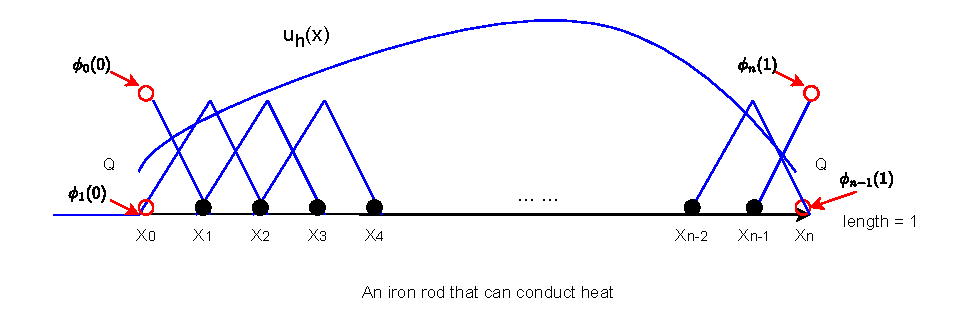
\includegraphics[width=15cm]{pic/1.1.pdf} % width设置图片大小
        \caption{The four annoying, non-differentiable points} % 设置图片的标题及引用标签
        \label{pic_3}
    \end{figure}
    \begin{figure}[H]
        \centering % 图片居中
        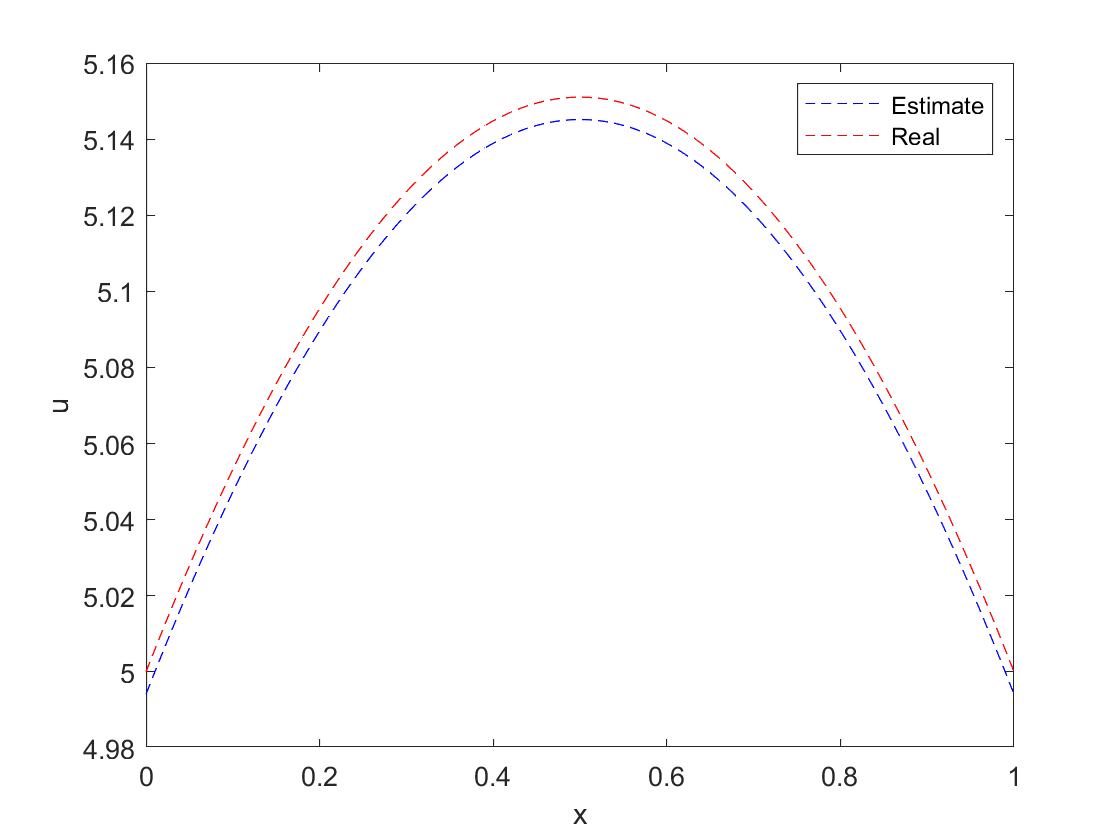
\includegraphics[width=12cm]{pic/result1.png} % width设置图片大小
        \caption{The final function curve graph, where the red line represents the real temperature distribution i.e. $u(x)$ while the blue represents the estimated one i.e. $u_h(x)$.} % 设置图片的标题及引用标签
        \label{pic_4}
    \end{figure}
    \subsection{A Further Problem}
    \subsubsection{Mathematical Derivation}
    In this chapter, we will focus on an opposite but more difficult question: suppose we have a known heat distribution $\hat{u}(x)$, while the internal heat source distribution $f(x)$ is unknown. Our goal is to find an approximation temperature distribution function \( u(x) \) and an internal heat source term f(x) that minimizes the difference between \( \hat{u}(x) \) and \( u(x) \) .

Mathematically, we want to solve the optimization problem:
\begin{equation}
\begin{cases}
    \min \frac{1}{2}||\hat{u}(x)-u(x)||^2_{2}+\frac{\phi}{2}||f(x)||^2_{2}\\
    \\
    s.t. -\frac{du^2}{d^2 x} - f(x) = 0 \label{convex basic} 
\end{cases}
\end{equation}
 The first term in the objective function $||\hat{u}(x)-u(x)||_2$ measures the difference between $u(x)$ and $\hat{u}(x)$, where the goal is obviously to decrease the difference between them. The second term in the objective function $\frac{\phi}{2}||f(x)||_2$ is a regularization term where somewhat small value is taken for $\phi$. Note that the objective function cannot be negative, thus the problem is well posed if the feasible set is not empty. The constraint function $ -\frac{du^2}{d^2 x} - f(x) = 0 $ is exactly from formula \ref{basic formula}, representing the influence of internal heat source on temperature distribution.

This formula \ref{convex basic} is rather a simple one, but hard to solve. Because what we need to solve are two unknown functions rather than variables. Using the similar thought of FEM in last chapter, we naturally associate it with the idea of subdividing unknown functions into grids and approximating them in the form of vectors. We discretize f(x), u(x) and $\hat{u}(x)$, making them to become vectors of n*1, recorded as f, u, and $\hat{u}$ :
\begin{equation}
\begin{cases}
    u = 
    \begin{pmatrix}
            u_1\\
            u_2\\
            ... ...\\
            u_n\\
    \end{pmatrix}\\
    \hat{u} = 
    \begin{pmatrix}
            \hat{u_1}\\
            \hat{u_2}\\
            ... ...\\
            \hat{u_n}\\
    \end{pmatrix}\\
    f = 
    \begin{pmatrix}
            f_1\\
            f_2\\
            ... ...\\
            f_n\\
    \end{pmatrix}\\
    
\end{cases}
\end{equation}


We have also applied some tricky improvements to make the optimization problem adapt to the discretized expression, resulting in a better fitting effect:

We use 'Weighted Norm' to replace the basic 'L2 norm' because it provides a more appropriate measure when considering the scale and weight of different variables. 
For weighted norm, we have 
\begin{equation}
||A||_M^2 = A^T*M*A
\end{equation}

So $||\hat{u}(x)-u(x)||^2_{2}$ and $||f(x)||^2_{2}$ change into $||\hat{u}-u||_M^2$ and $||f||_G^2$, where M and G are symmetric positive definite matrix, which define some norms. 

We also change the equation constraints into the stiffness matrix K, which we calculated in chapter 2, formula \ref{matrix form}.It may seem somewhat abrupt, as we do not appear to explicitly use the basis functions mentioned in the previous section. In fact, returning to the essence of the stiffness matrix, its core idea is to describe the system's response to external influences. Specifically, the elements of the stiffness matrix represent the relationship between temperature gradients and heat flux density. The larger the matrix elements, the higher the thermal conductivity in that direction. Regarding thermal coupling between nodes, the off-diagonal elements \(k_{ij}\) represent the degree of thermal coupling between node \(i\) and node \(j\), reflecting the heat conduction characteristics between nodes.
This Equivalent substitution reduces the optimal control problem \ref{convex basic} to be quadratic programming and becomes:

\begin{equation}
\begin{cases}
    \min \:\frac{1}{2}||\hat{u}-u||^2_{M}+\frac{\phi}{2}||f||^2_{G}\\
    \\
    s.t. \:K*u - f = 0  
\end{cases}
\end{equation}


The optimization problem described above now finally change into a typical convex optimization problem with equality constraints: the objective function is a quadratic convex function, and the constraints are defined as a convex set; the equality constraints are linear functions, also satisfying the requirements of convex functions. A classic method for solving standard convex optimization forms is the Lagrange multiplier method: by incorporating  constraint function multiplied by Lagrange multipliers $\lambda$ into the objective function. The final form is as follows:
\begin{equation}
     L(u,f,\lambda) = \frac{1}{2}||u-\hat{u}||^2_M+\frac{\phi}{2}||f||^2_{G}+\lambda^T(Ku-f)
\end{equation}
After unpacking the Weighted Norm, it becomes:
\begin{equation}
    L(u,f,\lambda) = \frac{1}{2}(u-\hat{u})^T M (u-\hat{u})+\frac{\phi}{2}f^TGf+\lambda^TKu-\lambda^Tf
\end{equation}


When the feasible region of a standard convex optimization problem is non-empty and satisfies the Slater condition, solving the problem can be equivalently transformed into solving the KKT (Karush-Kuhn-Tucker) conditions, meaning the KKT conditions are both necessary and sufficient for optimality. For KKT, we need to consider the feasibility conditions, stationary point conditions, dual feasibility (obviously), and complementary slackness conditions(obviously). For stationary point conditions, specifically, this can be viewed as taking the derivatives of the function \( L \) with respect to the three variables \( u \), \( f \), and \( \lambda \):
\begin{equation}
\begin{cases}
    \frac{\partial L}{\partial u} = M(u-\hat{u})+K^T\lambda=0\\
    \\
    \frac{\partial L}{\partial f} = \phi Gf-\lambda=0\\
    \\
    \frac{\partial L}{\partial \lambda} = Ku-f=0\\
\end{cases}
\end{equation}

After elimination and solving, we obtain the final answer:

\begin{equation}
\begin{cases}
    u = M^{-1}(M\hat{u}-K^T\lambda)\\
    f = \frac{1}{\phi}G^{-1}\lambda\\
    Ku-f=0
\end{cases}
\end{equation}

\begin{equation}
\begin{cases}
    u = \hat{u}-M^{-1}K^T(KM^{-1}u^T+\frac{1}{\phi}G^{-1})^{-1}K\hat{u}\\
    f = \frac{1}{\phi}G^{-1}(KM^{-1}K^T+\frac{1}{\phi}G^{-1})^{-1}K\hat{u}\\
    \lambda = (KM^{-1}K^T+\frac{1}{\phi}G^{-1})^{-1}K\hat{u}
\end{cases}
\end{equation}
    \subsubsection{Matlab Coding}
    After analyzing the theory in section 2.2.1, we wrote the corresponding MATLAB code. We assume the temperature distribution to be:
    \begin{equation}
    \hat{u}(x)=2\sin(4\pi x+\frac{3\pi}{2})+2
    \end{equation}
    The hyperparameters are decided to be $M=G=\mathbf{I}$, n=100 and $\phi=1$. We still use the basis functions defined in section 2.1, thus obtaining the same stiffness matrix K as the original one \ref{matrix form}. After substituting the stiffness matrix into the KKT equations, we obtain the final result as follows: the predicted temperature distribution is shown in Fig.\ref{tem_100}, and the predicted heat source distribution is shown in Fig.\ref{heat_100}. However, the fitting effect was not satisfactory since there is a big gap between the real temperature distribution and the fitting one.

    
    \begin{figure}[H]
        \centering % 图片居中
        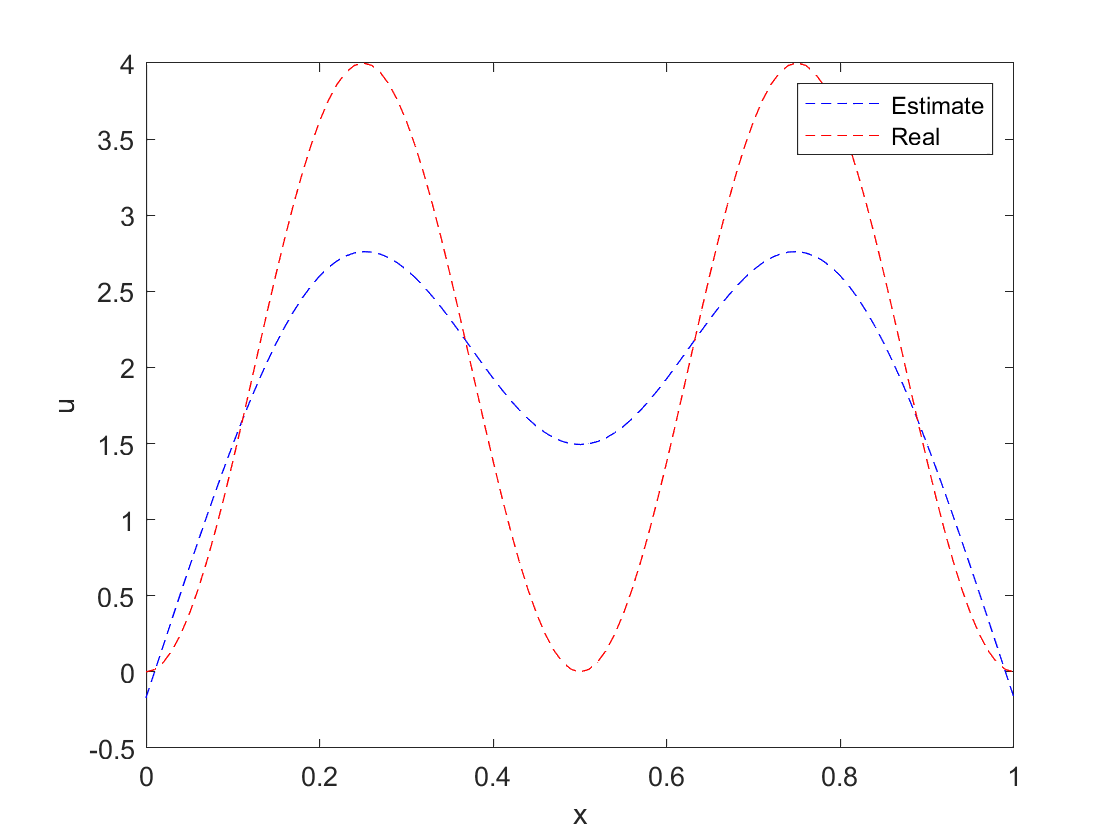
\includegraphics[width=12cm]{pic/n=100.png} % width设置图片大小
        \caption{Temperature distribution for n=100, where red line represents the real distribution, while the blue one is the fitting curve} % 设置图片的标题及引用标签
        \label{tem_100}
    \end{figure}
    \begin{figure}[H]
        \centering % 图片居中
        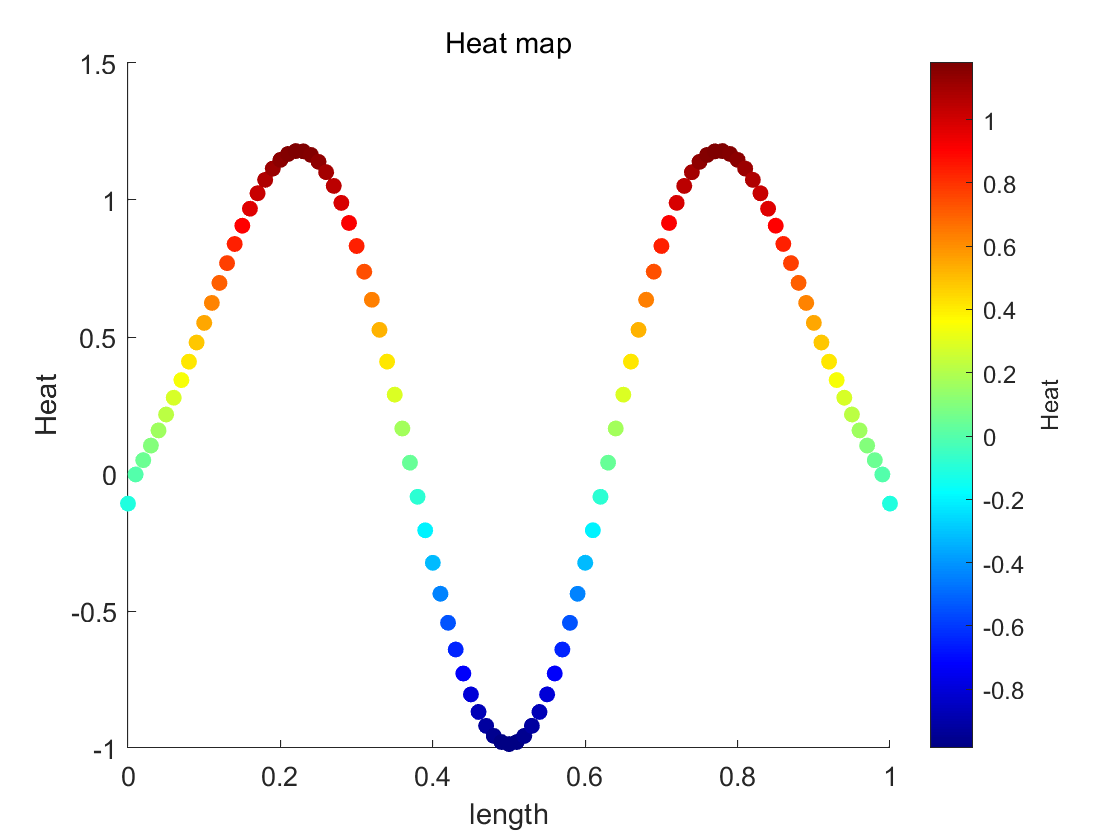
\includegraphics[width=12cm]{pic/f_n=100.png} % width设置图片大小
        \caption{The internal heat source distribution (vector) for n=100} % 设置图片的标题及引用标签
        \label{heat_100}
    \end{figure}
    The poor fitting performance may be caused by the following two aspects. Firstly, our choice of basis functions is too simplistic, which might lead to an inability to fit some complex curves, especially at points where the derivatives change significantly. Other common basis functions include Polynomial Basis Functions, trigonometric functions (sine and cosine functions), Radial Basis Functions, and so on. Secondly, we can further refine the segmentation, redesigning it from 100 segments to 500 segments. This will make our basis functions "slimmer and longer," allowing them to respond more sensitively to the features of the function and to be more sensitive to the conduction of internal heat sources.
    
     We refined the model, setting $n=500$ while keeping other parameters unchanged. The new stiff matrix now becomes five times larger. The results turn out to be much better: the predicted temperature distribution is shown in Fig.\ref{tem_500}, and the predicted heat source distribution is shown in Fig.\ref{heat_500}.
     
    \begin{figure}[H]
        \centering % 图片居中
        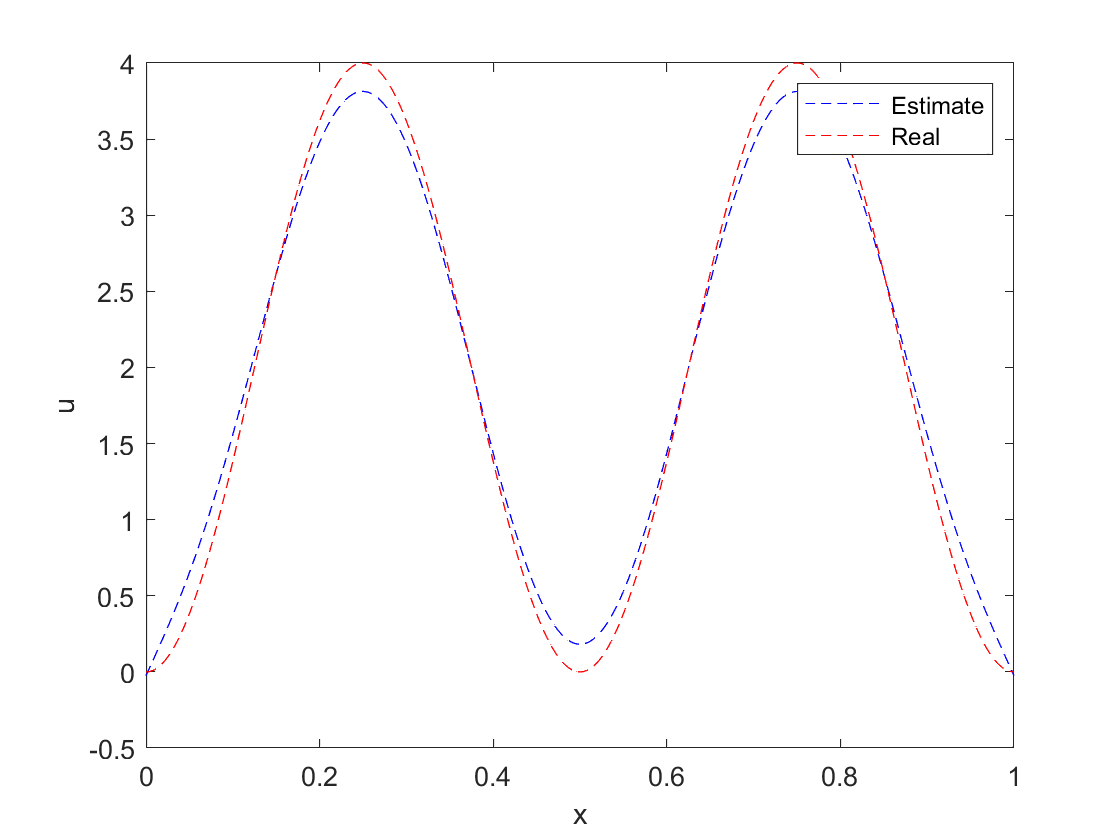
\includegraphics[width=11cm]{pic/n=500.png} % width设置图片大小
        \caption{Temperature distribution for n=500, where red line represents the real distribution, while the blue one is the fitting curve. Clearly shown, the fitting function better reflects the wavy and complex trends of the curve} % 设置图片的标题及引用标签
        \label{tem_500}
    \end{figure}        

    
    \begin{figure}[H]
        \centering % 图片居中
        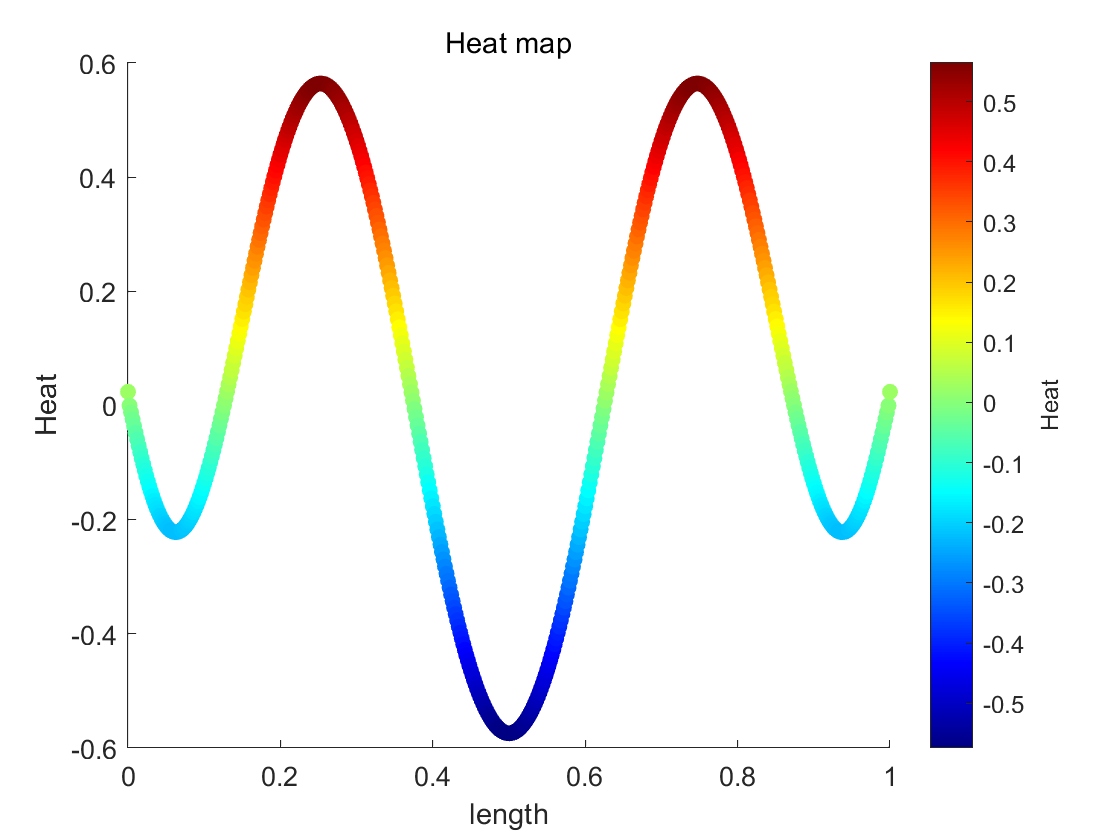
\includegraphics[width=10cm]{pic/f_n=500.png} % width设置图片大小
        \caption{The internal heat source distribution (vector) for n=500, compared to the previous distribution, it shows a clearer trend at both ends} % 设置图片的标题及引用标签
        \label{heat_500}
    \end{figure}
    
    \subsection{Final Problem}
    \subsubsection{A New Solution Approach Inspired By FETI}
    In this sector, we will step further into the problem raised in Chapter 2.2. That is: we have a known heat distribution $\hat{u}(x)$, while the internal heat source distribution $f(x)$ is unknown. Our goal is to find an approximation temperature distribution function \( u(x) \) and an internal heat source term f(x) that minimizes the difference between \( \hat{u}(x) \) and \( u(x) \). As the results shown in last Chapter, the fitting effect is not satisfactory, especially at points where the trend of the function curve changes significantly, i.e. points where the derivative changes significantly. The continuous refinement of the grid has indeed solved this problem to some extent, but it has also brought about an exponential increase in computing power. We need another refined approach to solve this problem, mainly manifested in smaller matrix calculations (especially inverse problems) and greater sensitivity to changes in internal heat sources.
    
    Base on this requirement, we will use a Finite Element Tearing and Interconnecting (FETI) - like method to solve this problem(\textcite{FETI1} and \textcite{FETI2}). FETI is a domain decomposition technique specifically designed for solving large-scale partial differential equations (PDEs). It operates by dividing the computational domain into smaller, non-overlapping subdomains, each of which can be solved independently. The solutions of these subdomains are then iteratively coordinated to ensure consistency across the entire domain. FETI is particularly advantageous in parallel computing environments and is well-suited for complex geometries and large-scale computational problems. Compared to single FEM, FETI effectively handles complex geometries and irregular domains without the need for uniform meshing across the entire domain, offering greater flexibility. Additionally, by imposing consistent boundary conditions at the subdomain interfaces, FETI naturally accommodates various complex boundary conditions, avoiding the complexity of handling boundary conditions in a global solution process(\textcite{more}).

    \subsubsection{Mathematical Derivation}
    In this chapter, we turn our attention to the FETI-like theory, attempting to cut the problem by independently handling each small segment and considering the mutual influence of each segment's boundaries. We re-examine our heat conduction problem in the iron rod: we first divide the iron rod into \(N_s\) segments,i.e. we get points $\{$$X^{0}$,$X^{1}$...$X^{Ns}$$\}$. Then, on each small segment, we independently apply FEM by dividing it again into \(n\) points. To take segment i as an example, we have: $\{$ $X^i_{0}$, $X^i_{1}$... $X^i_{n}$ $\}$. 
    
    The basic idea is shown as follow:
    \begin{figure}[H]
        \centering % 图片居中
        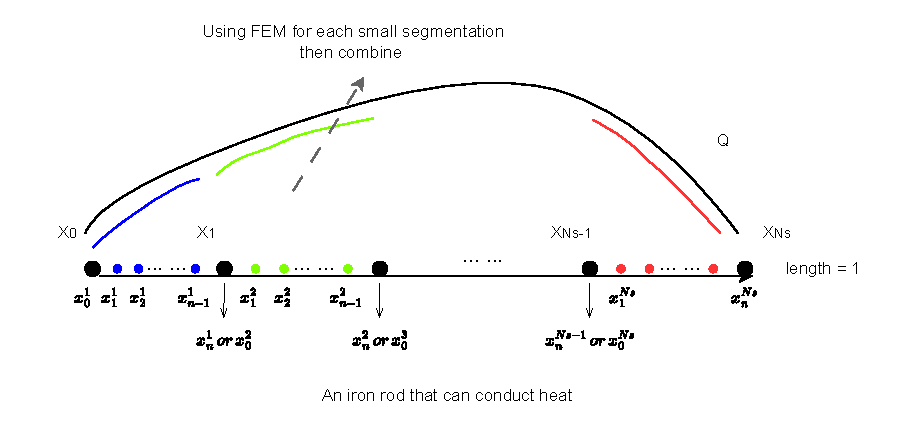
\includegraphics[width=15cm]{pic/2.drawio.pdf} % width设置图片大小
        \caption{The pole is first divided into Ns segments and then in each segment we again divide into n segments, just as what we have done in previous chapters. Then we do FEM in each small segment and get Ns stiffness matrices} % 设置图片的标题及引用标签
        \label{2}
    \end{figure}
    The formula \ref{convex basic} will now change into:
    \begin{equation}
        \begin{cases}
            min\:\: J(y,f,\lambda)=\frac{1}{2}\sum_{s=1}^{N_s}||u^s-\hat{u^s}||^2_{M^s}+\frac{1}{2}\sum_{s=1}^{N_s}\phi_{s}||f^s||^2_G+\frac{\phi_{\lambda}}{2}||\lambda||^2_G\\
            \\
            s.t. \:\:  K^s u^s = f^s + ({B^s_1+B^s_2)}^T\lambda \\
            \:\:\:\:\:\:\:\: constraints\, on\, \,segments'\, boundary
            \label{ffinal}
        \end{cases}
    \end{equation}
    Where $N_s$ is the number of subdomains, $u^s$ and $f^s$ are state variables and controlling force in the $s$-subdomain, respectively. $\lambda$ is extra control variables.
    
    Now consider the 'constraint on segments' boundary': $K^s$ is the stiffness matrix for each segment, while $\lambda$ is Lagrange multipliers and can be thought of as action-reaction forces between interconnecting surfaces. $B^s_i$ is a 1*(n+1) vector, where i $\in$ [1,2], representing the left or right end of the segmentation. To take the fist and second section as an example i.e. [$u^1_0$ ... $u^1_n$] and [$u^2_0$ ... $u^2_n$], the temperature of the right end of the first section should be the same as the left end of the second section, which means the nth point of $u^1$ should equal to 0th point of $u^2$. Thus, $B^2_1=[1,0...,0,0]$ and $B^2_2 = [0,0,0,...,-1]$ . Specially, the left side of 0th segmentation and the right end of the Ns segmentation should be equal to the given boundary conditions i.e. u(0) = u(1) = C. The constraints on segments' boundary can be written as follow:
    \begin{equation}
    constraints\, on\, segments' \,boundary = 
           % B_1^1 * u^1 = u^{1}_0 = C\\
            %B_2^{Ns} * u^{Ns} = u^{Ns}_n = C\\
            B^s_2u^s+B^{s+1}_{1}u^{s+1}=u^s_n-u^{s+1}_0=0 \:\:\: for\: s \in [1,Ns-1]
    \end{equation}
    Make $B^s=B^s_1+B^s_2$ and $(B^1_1=B^{N_s}_2=0)$ , B be a (2*Ns)*(n+1) matrix, where each line represent the relationship of adjacent end point.
    \begin{equation}
    B = 
        \begin{pmatrix}
            %[\:B^1_1\:]\\
            [\:B^1_2\:]\\
            [\:B^2_1\:]\\
            [\:B^2_2\:]\\
            ...\\
            [\:B^{Ns}_1\:]\\
            %[\:B^{Ns}_2\:]
        \end{pmatrix}
    \end{equation}
    Our objective function is clearly still a standard quadratic convex function with a convex set as its domain. The 2Ns constraints are all equality constraints and are linear, meeting the requirements for a convex function. Therefore, we can once again use the method of Lagrange multipliers and write out the corresponding KKT conditions.
    \begin{multline}
        L(u,f,\lambda,\mu,\gamma) = J(y,f,\lambda)+\sum_{s=1}^{Ns}\mu_s^T(K^su^s-f^s-{B^s}^T\lambda)+\sum_{s=1}^{Ns-1}{\gamma_s}^T(B^s_2 u^s+B^{s+1}_1u^{s+1})%+\gamma^0(B^1_1u^1-C) +\gamma^{Ns}%(B^{Ns}_2u^{Ns}-C)
    \end{multline}
    Where $\mu_s$ and $\gamma_s$ are lagrange multiplier vectors. The KKT forula should then be:
    Br = $B_2^{s^{T}} r_s + B_1^{s^{T}} r_{s-1}$\\
    \begin{equation}
        \begin{cases}
    \frac{\partial L}{\partial \gamma^s} = B^s_2 u^s + B^{s+1}_1 u^{s+1} = 0,\\
    \\
    %\frac{\partial L}{\partial \gamma^0} = B^1_1 u^1 - C = 0,\\
    %\\
    %\frac{\partial L}{\partial \gamma^{Ns}} = B^{Ns}_2 u^{Ns} - C %= 0,\\
    %\\
    \frac{\partial L}{\partial u^s} = M^s (u^s - \hat{u}^s) + {K^s}^T \mu^s + Br = 0,\\
    \\
    \frac{\partial L}{\partial f^s} = \phi_s G f^s - \mu_s = 0,\\
    \\
    \frac{\partial L}{\partial \lambda} = -\sum_{s=1}^{Ns} B^s \mu_s + \phi_\lambda G \lambda = 0,\\
    \\
    \frac{\partial L}{\partial \mu_s} = K^s u^s - f^s - {B^s}^T \lambda = 0.
    \label{long}
\end{cases}
\end{equation}

Using 2nd, 3th, and 4th formula in \ref{long}, we can get the solution be
$\Rightarrow $
    \\\begin{equation}
        \begin{cases}
        u^s = \hat{u}^s-M^{s^{-1}}({K^s}^T \mu^s + Br),\\
    \\
        f^s = \frac{1}{\phi_s}G^{-1}\mu^s,\\
    \\
        \lambda = \frac{1}{\phi_\lambda}G^{-1}\sum_{s=1}^{Ns} B^s \mu_s.
        \end{cases}
        \label{short}
 \end{equation}
 We now put the results back to the 1st and 5th formula in formula \ref{long}, and write the matrix form:


\begin{equation}
    \begin{bmatrix}
   A & C \\
   D & E
\end{bmatrix} 
*
\begin{bmatrix}
\mu_1 \\
\mu_2 \\
\vdots \\
\mu_{N_s}\\
\gamma_1 \\
\gamma_2 \\
\vdots \\
\gamma_{N_s-1} \\
\end{bmatrix} = \begin{bmatrix}
K^1 \hat{u}^1\\
K^2 \hat{u}^2 \\
\vdots \\
K^{N_s} \hat{u}^{N_s} \\
0 \\
0 \\
\vdots \\
0
\end{bmatrix}
\end{equation}

Where A, C, D, E matrices are defined as follow:

\begin{equation}
A = 
\begin{bmatrix}
A_1 & \frac{1}{\phi_\lambda} {B^1}^T G^{-1} B^2 & \frac{1}{\phi_\lambda} {B^1}^T G^{-1} B^3 & \cdots & \frac{1}{\phi_\lambda} {B^1}^T G^{-1} B^{N_s} \\
\frac{1}{\phi_\lambda} {B^2}^T G^{-1} B^1 & A_2 & {\phi_\lambda} {B^2}^T G^{-1} B^{3} & \cdots & \frac{1}{\phi_\lambda} {B^2}^T G^{-1} B^{N_s} \\
\frac{1}{\phi_\lambda} {B^3}^T G^{-1} B^1  & {\phi_\lambda} {B^3}^T G^{-1} B^{2} & A_3 & \cdots & \frac{1}{\phi_\lambda} {B^3}^T G^{-1} B^{N_s} \\
\vdots & \vdots & \vdots & \ddots & \vdots \\
\frac{1}{\phi_\lambda} {B^{N_s}}^T G^{-1} B^1 & \frac{1}{\phi_\lambda} {B^{N_s}}^T G^{-1} B^2 & \frac{1}{\phi_\lambda} {B^{N_s}}^T G^{-1} B^3 & \cdots & A_{N_s} 
\end{bmatrix}
\end{equation}
 Let $A_i = K^i M^{i^{-1}} K^{i^{T}} + \frac{1}{\phi_i} G^{-1} + \frac{1}{\phi_\lambda} {B^i}^T G^{-1} B^i $

\begin{multline}
\\\tiny
C = 
\begin{bmatrix}
K^1 M^{1^{-1}} B_2^{1^{T}} & K^2 M^{2^{-1}} B_1^{2^{T}} & 0 & \cdots & 0\\
 0 & K^2 M^{2^{-1}} B_2^{2^{T}} & K^3 M^{3^{-1}} B_1^{3^{T}} & \cdots & 0 & 0\\
 0 & 0 & K^3 M^{3^{-1}} B_2^{3^{T}} & \cdots & 0 & 0\\
 \vdots & \vdots & \vdots & \ddots & \vdots & \vdots \\
0 & 0 & 0 & \cdots & K^{N_s-1} M^{{N_s-1}^{-1}} B_2^{{N_s-1}^{T}} & K^{N_s} M^{{N_s}^{-1}} B_1^{{N_s}^{T}}\\
\end{bmatrix}
\\
D =
\begin{bmatrix}
B^1_2 M^{1^{-1}} K^{1^{T}} &  B^2_1 M^{2^{-1}} K^{2^{T}} & 0 & \cdots & 0 & 0 \\
0 & B^2_2 M^{2^{-1}} K^{2^{T}} & B^3_1 M^{3^{-1}} K^{3^{T}} & \cdots & 0 & 0 \\
 \vdots & \vdots & \vdots & \ddots & \vdots & \vdots \\
 0 & 0 & 0 & \cdots & B^{N_s-1}_2 M^{{N_s-1}^{-1}} K^{{N_s-1}^{T}} &  B^{N_s}_1 M^{{N_s}^{-1}} K^{{N_s}^{T}} 
\end{bmatrix}
\\
E = 
\begin{bmatrix}
E_1 & B^2_1 M^{2^{-1}} B_2^{2^{T}} & 0 & \cdots & 0 & 0 \\
 B^2_2 M^{2^{-1}} B_1^{2^{T}} & E_2 & B^3_1 M^{3^{-1}} B_2^{3^{T}} & \cdots & 0 & 0 \\
 \vdots & \vdots & \vdots & \ddots & \vdots & \vdots \\
  0 & 0 & 0 & \cdots & B^{N_s-2}_2 M^{{N_s-2}^{-1}} B_1^{{N_s-2}^{T}} &  E_{Ns-1}
\end{bmatrix}
\end{multline}
Where 
\begin{equation}
    E_i = B^i_2 M^{i^{-1}} B_2^{i^{T}} + B^{(i+1)}_1 M^{{(i+1)}^{-1}} B_1^{{(i+1)}^{T}}
\end{equation}


\subsubsection{Matlab Coding}
 In the MATLAB test, we still assume the real temperature distribution to be     \begin{equation}
    \hat{u}(x)=2\sin(4\pi x+\frac{3\pi}{2})+2
    \end{equation}
    the hyperparameters are decided to be $M=G=\mathbf{I}$, which implies uniform weighting of the state variables, i.e. we assume that the errors at different points along the rod have the same impact on the fitting (we will try other matrices in following chapter). And $\phi_s=\phi_\lambda=1$.
   Since FETI can divide the entire region into multiple independent subdomains and applying FEM characteristics in different subdomains. FETI can indeed handle complex and irregular distribution shapes better and provide more accurate fitting results. To prove this conclusion, we use two different Ns. First, we divided the entire region into $N_s = 5$ subdomains, with each subdomain divided into $20$ segments, this ensures the equal segmentation number as defined in the fist situation in last chapter i.e. n = 100. The result are shown in figure \ref{se_100}, which is much better than the result under the same condition in section 2.2 \ref{tem_100}. Then, we divided the entire region into $N_s = 5$ subdomains, with each subdomain divided into $100$ segments. The result are shown in figure \ref{se_500}, which also indicates enormous improvement in fitting complex distribution compared to method in the second situation in section 2.2 \ref{tem_500}.
    \begin{figure}[H]
        \centering % 图片居中
        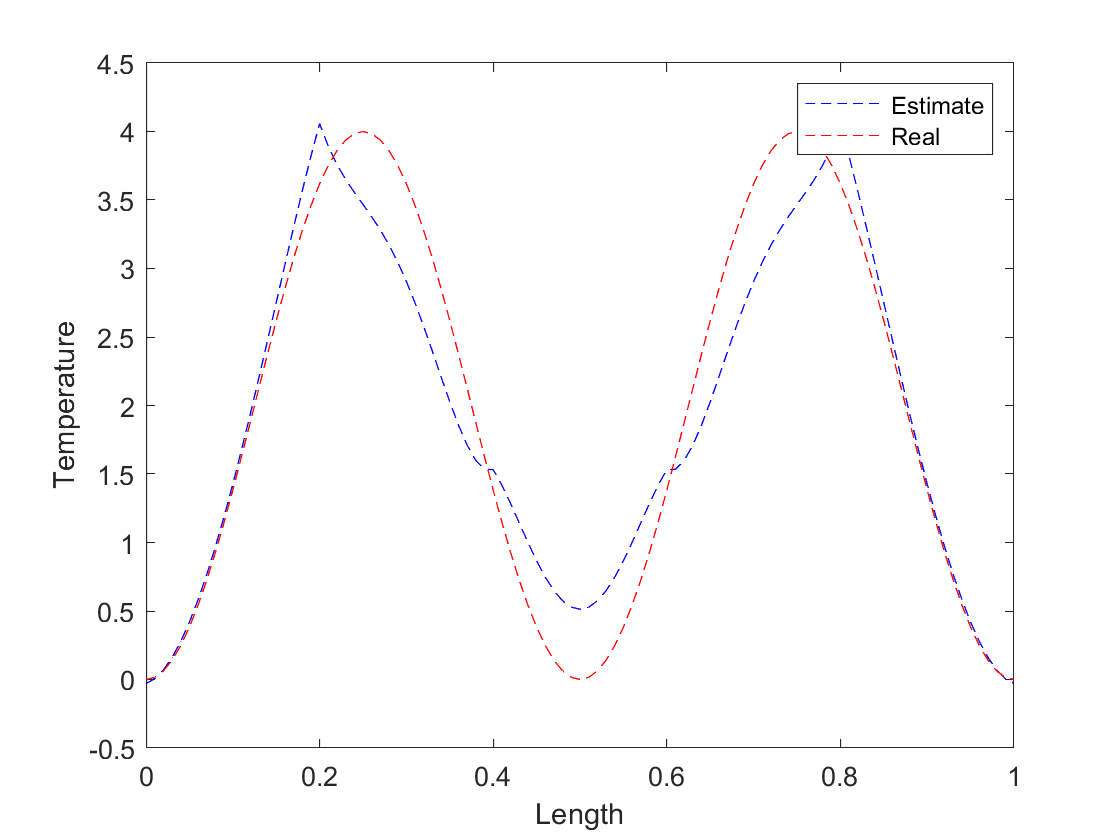
\includegraphics[width=11cm]{pic/se3_n=100.png} % width设置图片大小
        \caption{Temperature distribution for $N_s=5$ subdomains and $N=20$ segments in each subdomain, where red line represents the real distribution, while the blue one is the fitting curve.} % 设置图片的标题及引用标签
        \label{se_100}
    \end{figure}     
    \begin{figure}[H]
        \centering % 图片居中
        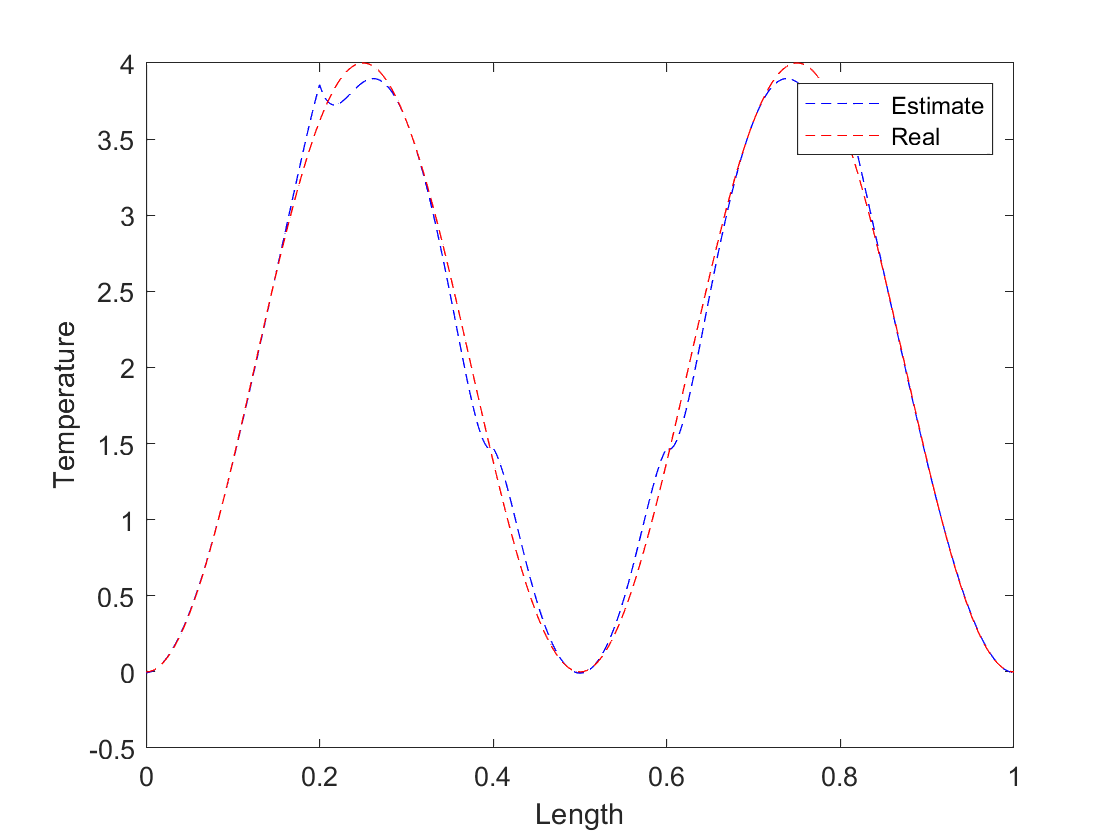
\includegraphics[width=11cm]{pic/se3_n=500.png} % width设置图片大小
        \caption{Temperature distribution for $N_s=5$ subdomains and $N=100$ segments in each subdomain, where red line represents the real distribution, while the blue one is the fitting curve.} % 设置图片的标题及引用标签
        \label{se_500}
    \end{figure}    
\section{Exploration Of Some Hyperparameters}
In this chapter, we will explore some hyperparameters based on formula \ref{ffinal}, committed to achieving the best fitting results.Using the control variable method, we only change one parameter at a time, where other parameters are keep the same with result \ref{se_500}.
\subsection{The Impact Of $\phi_s$ On The Fitting Effect}
We start with 1, increase with step size of 10 and gradually achieve 1000, exploring the influence of the weight of the internal heat element f(x) distribution on the fitting effect. It has been proven that increasing the weight hardly improves the fitting effect, which should be due to the fact that the most basic thermodynamic formula determines the decisive effect of the distribution of internal heat sources on temperature distribution, and the two are inherently strongly correlated.
 \begin{figure}[H]
        \centering % 图片居中
        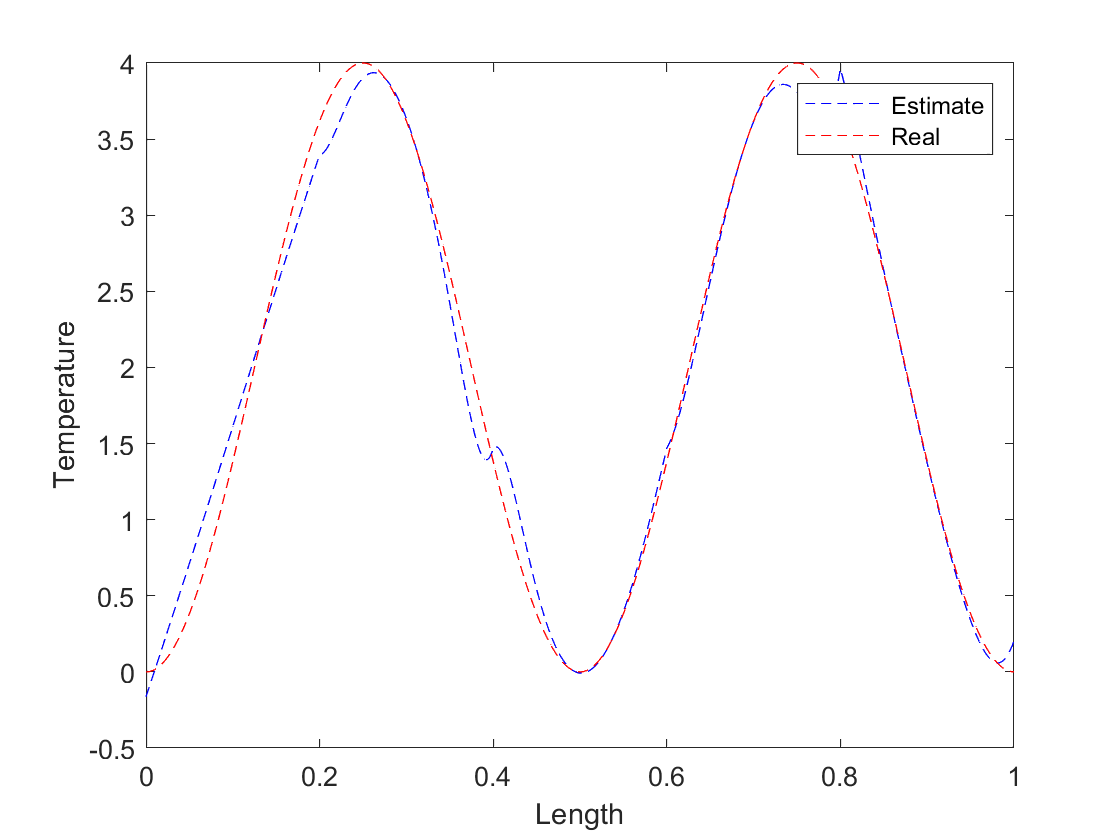
\includegraphics[width=11cm]{pic/phi_s=1000.png} % width设置图片大小
        \caption{We provide a extreme case where $\phi_s$ is 1000, and it has been proven that this has little impact on the result} % 设置图片的标题及引用标签
        \label{phi_s=1000}
    \end{figure}     
\subsection{The impact of $\phi_{\lambda}$ On The Fitting Effect}
$\phi_{\lambda}$ primarily controls the influence weight of the hyperparameter $\lambda$ on the optimization of the objective function. $\lambda$ is an important parameter in the constraint function for controlling the B matrix, specifically the transition constraints between different segments.

We still start with 1, increase with step size of 10 and gradually achieve 1000. The result of $\phi_\lambda$ =1000 is as follow:
 \begin{figure}[H]
        \centering % 图片居中
        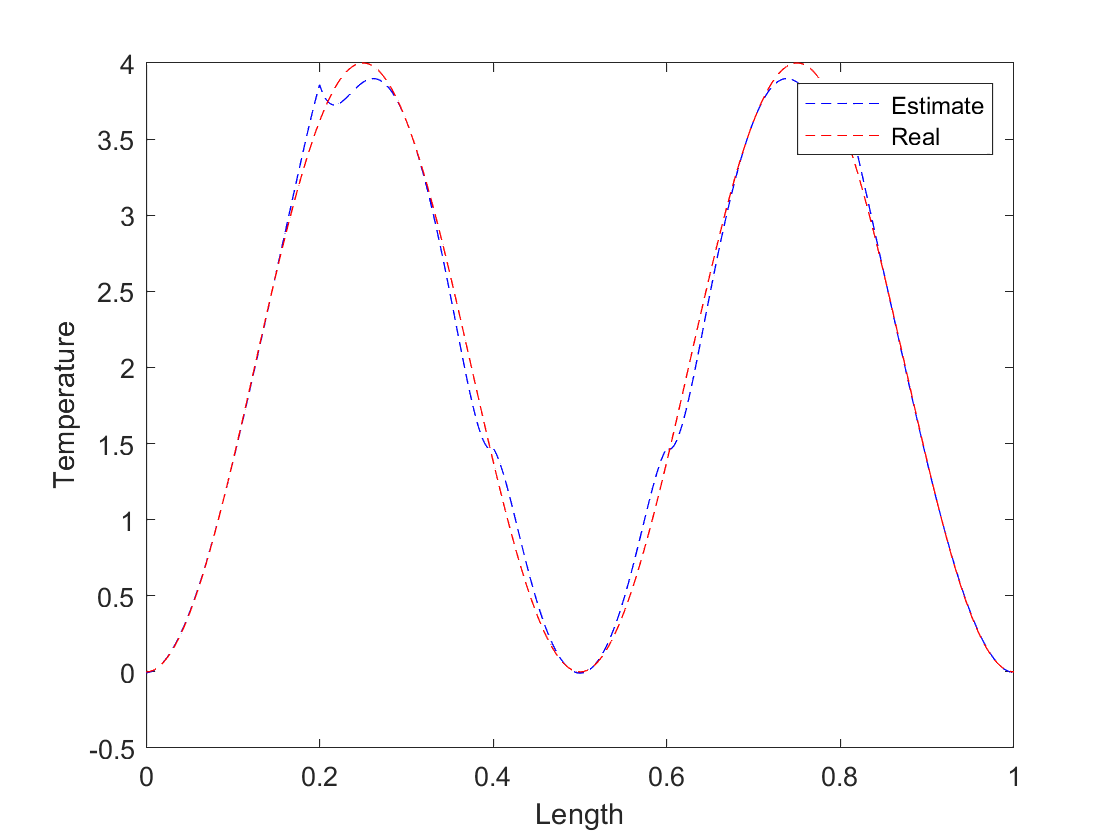
\includegraphics[width=11cm]{pic/phi_lambda=1000.png} % width设置图片大小
        \caption{We provide a extreme case where $\phi_\lambda$ is 1000, and it has been proven that this has little impact on the result} % 设置图片的标题及引用标签
        \label{phi_l=1000}
    \end{figure} 
\subsection{The Impact Of Weighted Norm On The Fitting Effect}
The weighted norm, i.e. M and G matrices also playes an important role in our objective funtion \ref{ffinal}, in the previous chapter we simply define them as Identity matrix, which implies uniform weighting of the state variables, i.e. we
assume that the errors at different points along the rod have the same impact on the fitting. Now we will change the matrix into a more complex one.
The two tricky designs are as follow:
the first matrix's diagnal elements are [0,10,20,...,490,500,490,...,10,0]and second's are 
[500,490,480,...,10,0,10,...,490,500]. We actually get a much better result, this is because the real temperature is distributed unevenly, so if we pay more attention to the undulating part, we might fit better:
 \begin{figure}[H]
        \centering % 图片居中
        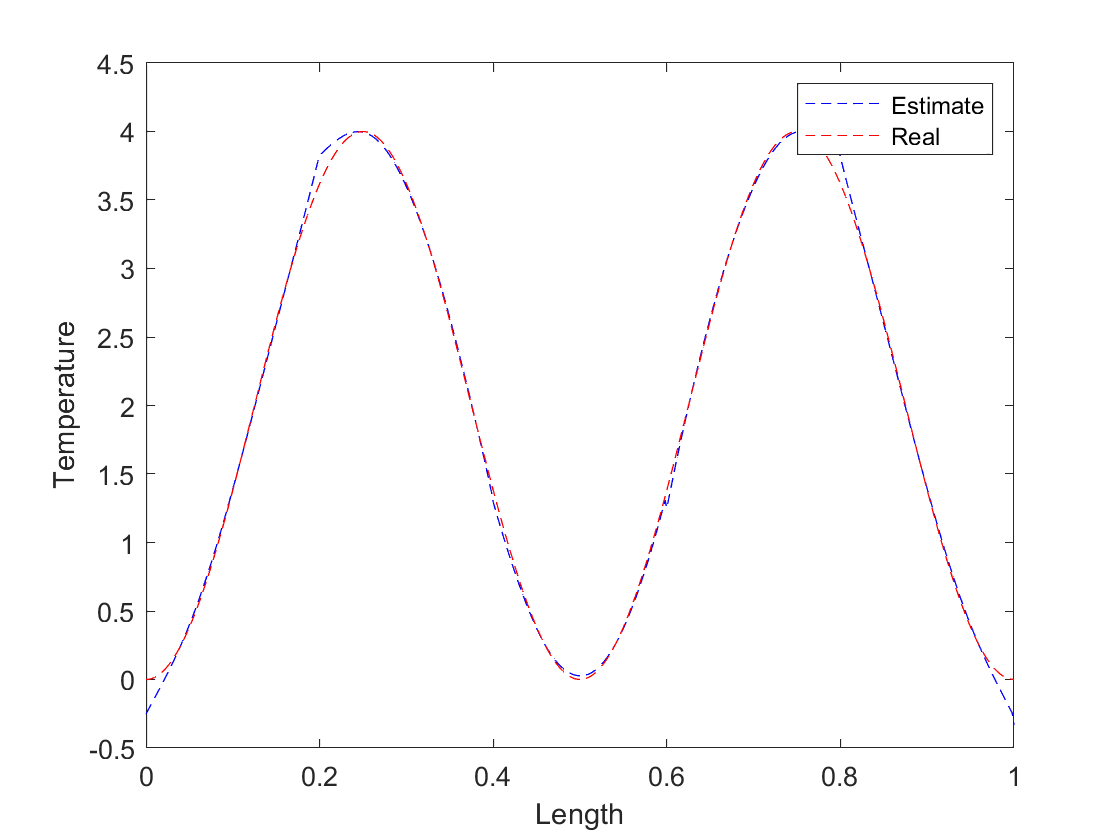
\includegraphics[width=11cm]{pic/mid_high.png} % width设置图片大小
        \caption{The diagonal elements of a symmetric matrix are now increasing from two diagonals to the middle} % 设置图片的标题及引用标签
        \label{m1=1000}
    \end{figure} 
    
 \begin{figure}[H]
        \centering % 图片居中
        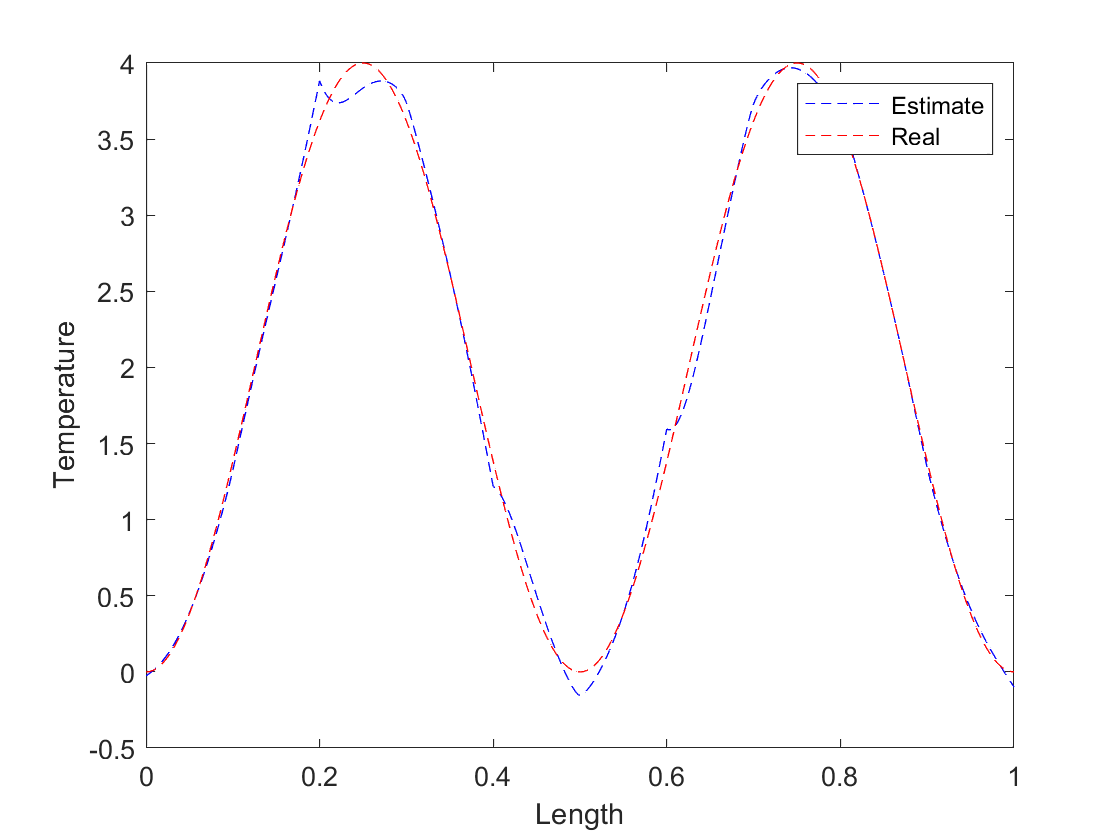
\includegraphics[width=11cm]{pic/mid_low.png} % width设置图片大小
        \caption{The diagonal elements of a symmetric matrix are now decreasing from two diagonals to the middle} % 设置图片的标题及引用标签
        \label{m2=1000}
    \end{figure} 

\section{Possible Improvements and Future Prospects}
Although our study demonstrates significant progress, there are still some innovative improvements that await further exploration and research:
\begin{enumerate}
    \item In terms of the basis function settings, the simplicity and "sharpness" of our basis functions lead to imperfect fitting results. Although we tried smoother functions such as sine functions as replacements, we did not achieve satisfactory results. However, we believe that more reasonable basis function designs (more complex, more categorized discussions, and smoother curve trends) can yield better results.
    \item For boundary conditions, we used the simplest constant constraints. In reality, the constraints at both ends should not be in the form of "points." In other words, if we force the two ends of the conductor to contact absolute temperatures, thereby controlling the endpoint temperatures, the impact should involve the entire conductor.
    \item In this paper, we consistently set the thermal conductivity (k) to a constant value of 1. However, for more complex problems, the thermal conductivity of the conductor may be a function related to position, i.e., \(k(x)\).
    \item Our computational power was severely tested in solving the second and third questions, especially when dealing with a large number of matrix inversions or matrix derivatives. In fact, for matrix operations, there are many tricky solution ideas, such as parallel computing or customized programming for specific problems.
    \item Currently, we are still manually adjusting the parameters of the weighted norm, specifically M and G. However, once we confirm its effectiveness, it is theoretically possible to implement automatic dynamic adjustments based on the actual distribution. Given the characteristics of our actual distribution, we should always be able to find the optimal norm method.\cite{anonymous2024sophiainaudition}
\end{enumerate}

\section{Conclusion}
Through the in-depth exploration of the three aforementioned problems, we tackled the issue of heat conduction in thermodynamics. Starting from the most fundamental FEM solutions, we discretized the problems to combine FEM with optimization algorithms, ultimately extending to the FETI concept. We successfully addressed the fitting problem of temperature distribution on conductors and the estimation problem of internal heat sources. We have explored various possible combined applications based on the finite element method and analyzed the impact of various factors on the results as much as possible. Our final result is pleasing and satisfactory

The entire process, from topic selection to final draft, took over one and a half months. Our thorough research allowed us to fully understand the core concepts of Finite Elements and various subsequent derivative algorithms. In the third chapter, we attempted to derive many different approaches based on existing papers. However, due to our limited mathematical and coding capabilities, we ultimately agreed on and implemented the best algorithm within our reach: FETI. However, the methods we attempted and the literature we reviewed behind the scenes are far more extensive than what is presented in the paper.

Throughout this paper, we successfully integrated several courses, such as Numerical Optimization, Convex Optimization, and Computational Science and Engineering. The sense of unreality brought about by purely theoretical derivations in class was completely resolved. We sincerely thank the professor for the hard work and excellent teaching this semester, this project has also brought us considerable gains. As a group from CS, we experienced the joy of combining mathematics and programming. Compared to the traditional purpose-driven programming in professional courses, this model, where mathematical design and programming complement each other, allowed us to appreciate the freedom and creativity of going from 0 to 1. As mentioned earlier, there are still many areas for improvement in our paper due to time and ability. We hope to further refine our work in future research. Lastly, we sincerely thank you for your patient reading. Just as we have poured a great deal of passion and effort into this paper, we hope that you will also find it rewarding and enjoyable. Thank you!
\printbibliography
\end{document}
